\documentclass[tikz]{standalone}
%\usetikzlibrary{...}% tikz package already loaded by 'tikz' option
\usepackage{amssymb}
\begin{document}
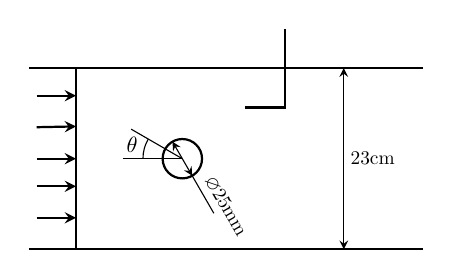
\begin{tikzpicture}[thick, scale=0.1]% Example:

    % limites de la veine
    \draw (-10,0) -- (40,0);
    \draw (-10,23) -- (40,23);

    % sonde de pitot
    \draw (17.5,18) -- (22.5,18) -- (22.5,28);

    % cylindre
    \draw (9.5,11.5) circle (2.5);

    % écoulement
    \draw (-4,0) -- (-4,23);
    \draw[->,>=stealth] (-9, 4) -- (-4, 4);
    \draw[->,>=stealth] (-9, 8) -- (-4, 8);
    \draw[->,>=stealth] (-9, 11.5) -- (-4, 11.5);
    \draw[->,>=stealth] (-9, 15.5) -- (-4, 15.6);
    \draw[->,>=stealth] (-9, 19.5) -- (-4, 19.5);

    % theta
    \draw[thin] (2,11.5) -- (9.5,11.5);
    \draw[thin, shift={(9.5,11.5)}] (0,0) -- (-30:-7.5);
    \draw[thin, shift={(9.5,11.5)}] (-5,0) arc (180:150:5);
    \draw[thin, shift={(9.5,11.5)}] (-20:-5) node[left,scale=0.8] {$\theta$};

    % dimensions
    %% veine
    \draw[thin, <->, >=stealth] (30,0) -- (30,23) node[midway,right, scale=0.7] {23cm};
    %% cylindre
    \draw[thin, shift={(9.5,11.5)}, <->, >=stealth] (-60:-2.5) -- (-60:2.5);
    \draw[thin, shift={(9.5,11.5)}] (-60:2.5) -- (-60:8) node[rotate=-60, scale=0.7, above] {$\varnothing$25mm};


\end{tikzpicture}
\end{document}
